

% quantum impurity problem,  boundary critical phenomena, Anderson orthogonality catastrophe
In (one-dimensional) quantum critical systems, the presence of physical boundary and isolated impurity weakly break the conformal symmetry. Simply put, they scatter and hence relate the otherwise independent modes and therefore demonstrate novel boundary critical phenomena\cite{cardy_boundary_2004}. Operators close to the boundary are interpreted as boundary condition changing operator\cite{oshikawa_boundary_1997,affleck_boundary_1997} in the boundary conformal field theory (CFT). Their correlation functions exhibit different critical exponent from the bulk\cite{cardy_conformal_1984}. One example is the "Anderson orthogonality catastrophe", where the core hole creates a potential that act as an impurity to the conduction band. The X-ray absorption rate will then have a power singularity of boundary exponent\cite{affleck_boundary_1997} at the resonance frequency. There are numerous impurity problem of this kind that has been studied in the last few decades, such as magnetic impurity in spin chain\cite{eggert_magnetic_1992}, boundary and impurity effects in Luttinger liquid\cite{fabrizio_interacting_1995}, entanglement of the defects\cite{peschel_entanglement_2005, igloi_entanglement_2009,calabrese_entanglement_2012} \etc

% non-equilibrium dynamics, particle mediate the two parts, Cardy cut-and-join protocol, Vassur majarana
Recently, more attention has been paid to the non-equilibrium dynamics of the quantum impurity. The "cut-and-join" quench protocol is a popular framework to study the spreading of influence from the localized impurity (or boundary) cross the system. As shown in Fig.~\ref{fig:cut-and-join}, one first prepares the ground states of the critical chain A and B, and then connect them at $t = 0$ and evolve. Various quantities are used to detect the information in the quench process. For instance, Ref.~\onlinecite{calabrese_entanglement_2007, calabrese_quantum_2016} find a logarithmic increase of entanglement entropy in subsystem $A$, when both $A$ and $B$ are identical critical systems. And the authors ascribe the growth to the proliferation and propagation of quasi-particle excitation emitted at the joint. Ref.~\onlinecite{vasseur_universal_2014} take A to be a normal lead and B to be a topological superconductor in topological phase and calculate the Loschmidt echo (overlap of wavefunction, see below) of the evolution. In this mode, effectively it is the Majorana zero mode which mediates the left and right modes of the free fermion that are responsible for the universal power law decay of the Loschmidt echo with the boundary critical exponent. 

\begin{figure}[htb]
\centering
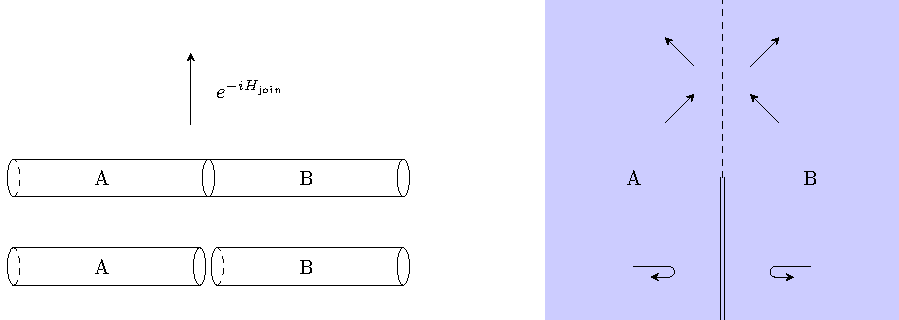
\includegraphics[width=\textwidth]{fig_cut_and_join.pdf}
\caption{Cut-and-join quench protocol. Left panel: prepare the ground states of two separated chains and joined them at $t = 0$, then do the time evolution with whole chain Hamiltonian. Right panel: spacetime diagram of the cut and join protocol. The solid line represents the boundaries of the two disconnected chains. It is totally reflective for the incident particles on both sides. The dashed line is the world line of the junction, which we will call interface. It could either be totally transparent or partially permeable, depending the types of theories of A and B.}
\label{fig:cut-and-join}
\end{figure}

% All of these are the same CFTs. we consider different CFTs, the mediating particle or primary field will be different, from the S matrix point of view.
In the path integral language, the "cut-and-join" protocol corresponds to a spacetime diagram as shown in Fig.~\ref{fig:cut-and-join}. The separating ground stats prepared before $t = 0$ are joined to form a new type of interface between them. Before the quench, the slit before $t = 0$ represents the boundary that are completely reflective to the injecting particles. The joining turns on the transmission from one side to the other. In the entanglement entropy and Loschmidt echo examples cited above\cite{calabrese_entanglement_2007, calabrese_quantum_2016, vasseur_universal_2014}, the two sides of the CFTs are the same (chiral fermion CFT in the case of \onlinecite{vasseur_universal_2014}) and the boundary becomes totally transparent after the joining. 

It would therefore be interesting to consider to connect two different CFTs in the "cut-and-join" protocol. The interface produced will interpolate between the total reflective and complete transparent ones. It can be realized as interface of two free compact Boson theories with different compactification radii\cite{bachas_permeable_2002}. There is also non-compact free boson/free fermion lattice realization, which was used to numerically and analytically\cite{peschel_exact_2012,sakai_entanglement_2008} study entanglement properties. In these models, there is a parameter $\lambda$ that is directly related to the transmission coefficient. In the compact Boson case, it is controlled by the ratio of the compactification radii and in the free lattice Boson case by ratio of masses. We expect it to be tunable in the a realistic experimental setting.

% fidelity and Loschmidt echo are quantities that extract boundary critical exponents, may reveal the nature of the mediating particle 
Fidelity and Loschmidt echo are the two quantities we compute to extract information from the quench process. Fidelity is the (square of) the overlap of the ground state wavefunction of the Hamiltonian before and after the quench. There is no dynamic information in fidelity, nevertheless its finite size effect also reveal the boundary critical exponent that maybe be diagnostic in Loschmidt echo computation. The Loschmidt echo is (square of) the overlap of the wavefunction before the quench and the one evolved at time $t$. The Loschmidt echo decays with a power law for the lack of length scale in the $t \rightarrow \infty$ limit. Its exponent has been calculated for various geometries and combinations of normal boundary conditions of the same CFT in \onlinecite{stephan_logarithmic_2013,stephan_local_2011}. What we do in this paper is to extend the analysis to the aforementioned parametric interface of (possibly) different CFTs. 

% structure of the paper.
\todo[inline]{structure of the paper}

%%% Local Variables:
%%% TeX-master: "bCFT_paper"
%%% TeX-PDF-mode: t
%%% End:
